% chapters/03_hardware_design.tex - Chapter 3: Hardware Design
% =============================================================

\chapter{Mechanical \& Electrical Design}
\label{chap:hardware-design}

This chapter describes the hardware components, electrical systems, and physical assembly of the Rescue Rover. The design prioritizes modularity, repairability, and use of readily available components. Each subsystem is documented with specifications, selection rationale, and integration considerations.

% --------------------------------------------------------
\section{Design Philosophy}
\label{sec:design-philosophy}

The hardware design follows three guiding principles. First, all components must be purchasable from common suppliers without lead times. Second, the system must be repairable using basic tools and without specialized equipment. Third, interfaces between modules must use standard connectors and protocols to allow future upgrades.

These constraints led us to select development boards over custom PCBs, through-hole components over surface mount where possible, and dupont wire connections over soldered joints for early prototypes.

% FIGURE PLACEHOLDER
\begin{figure}[h!]
    \centering
    % 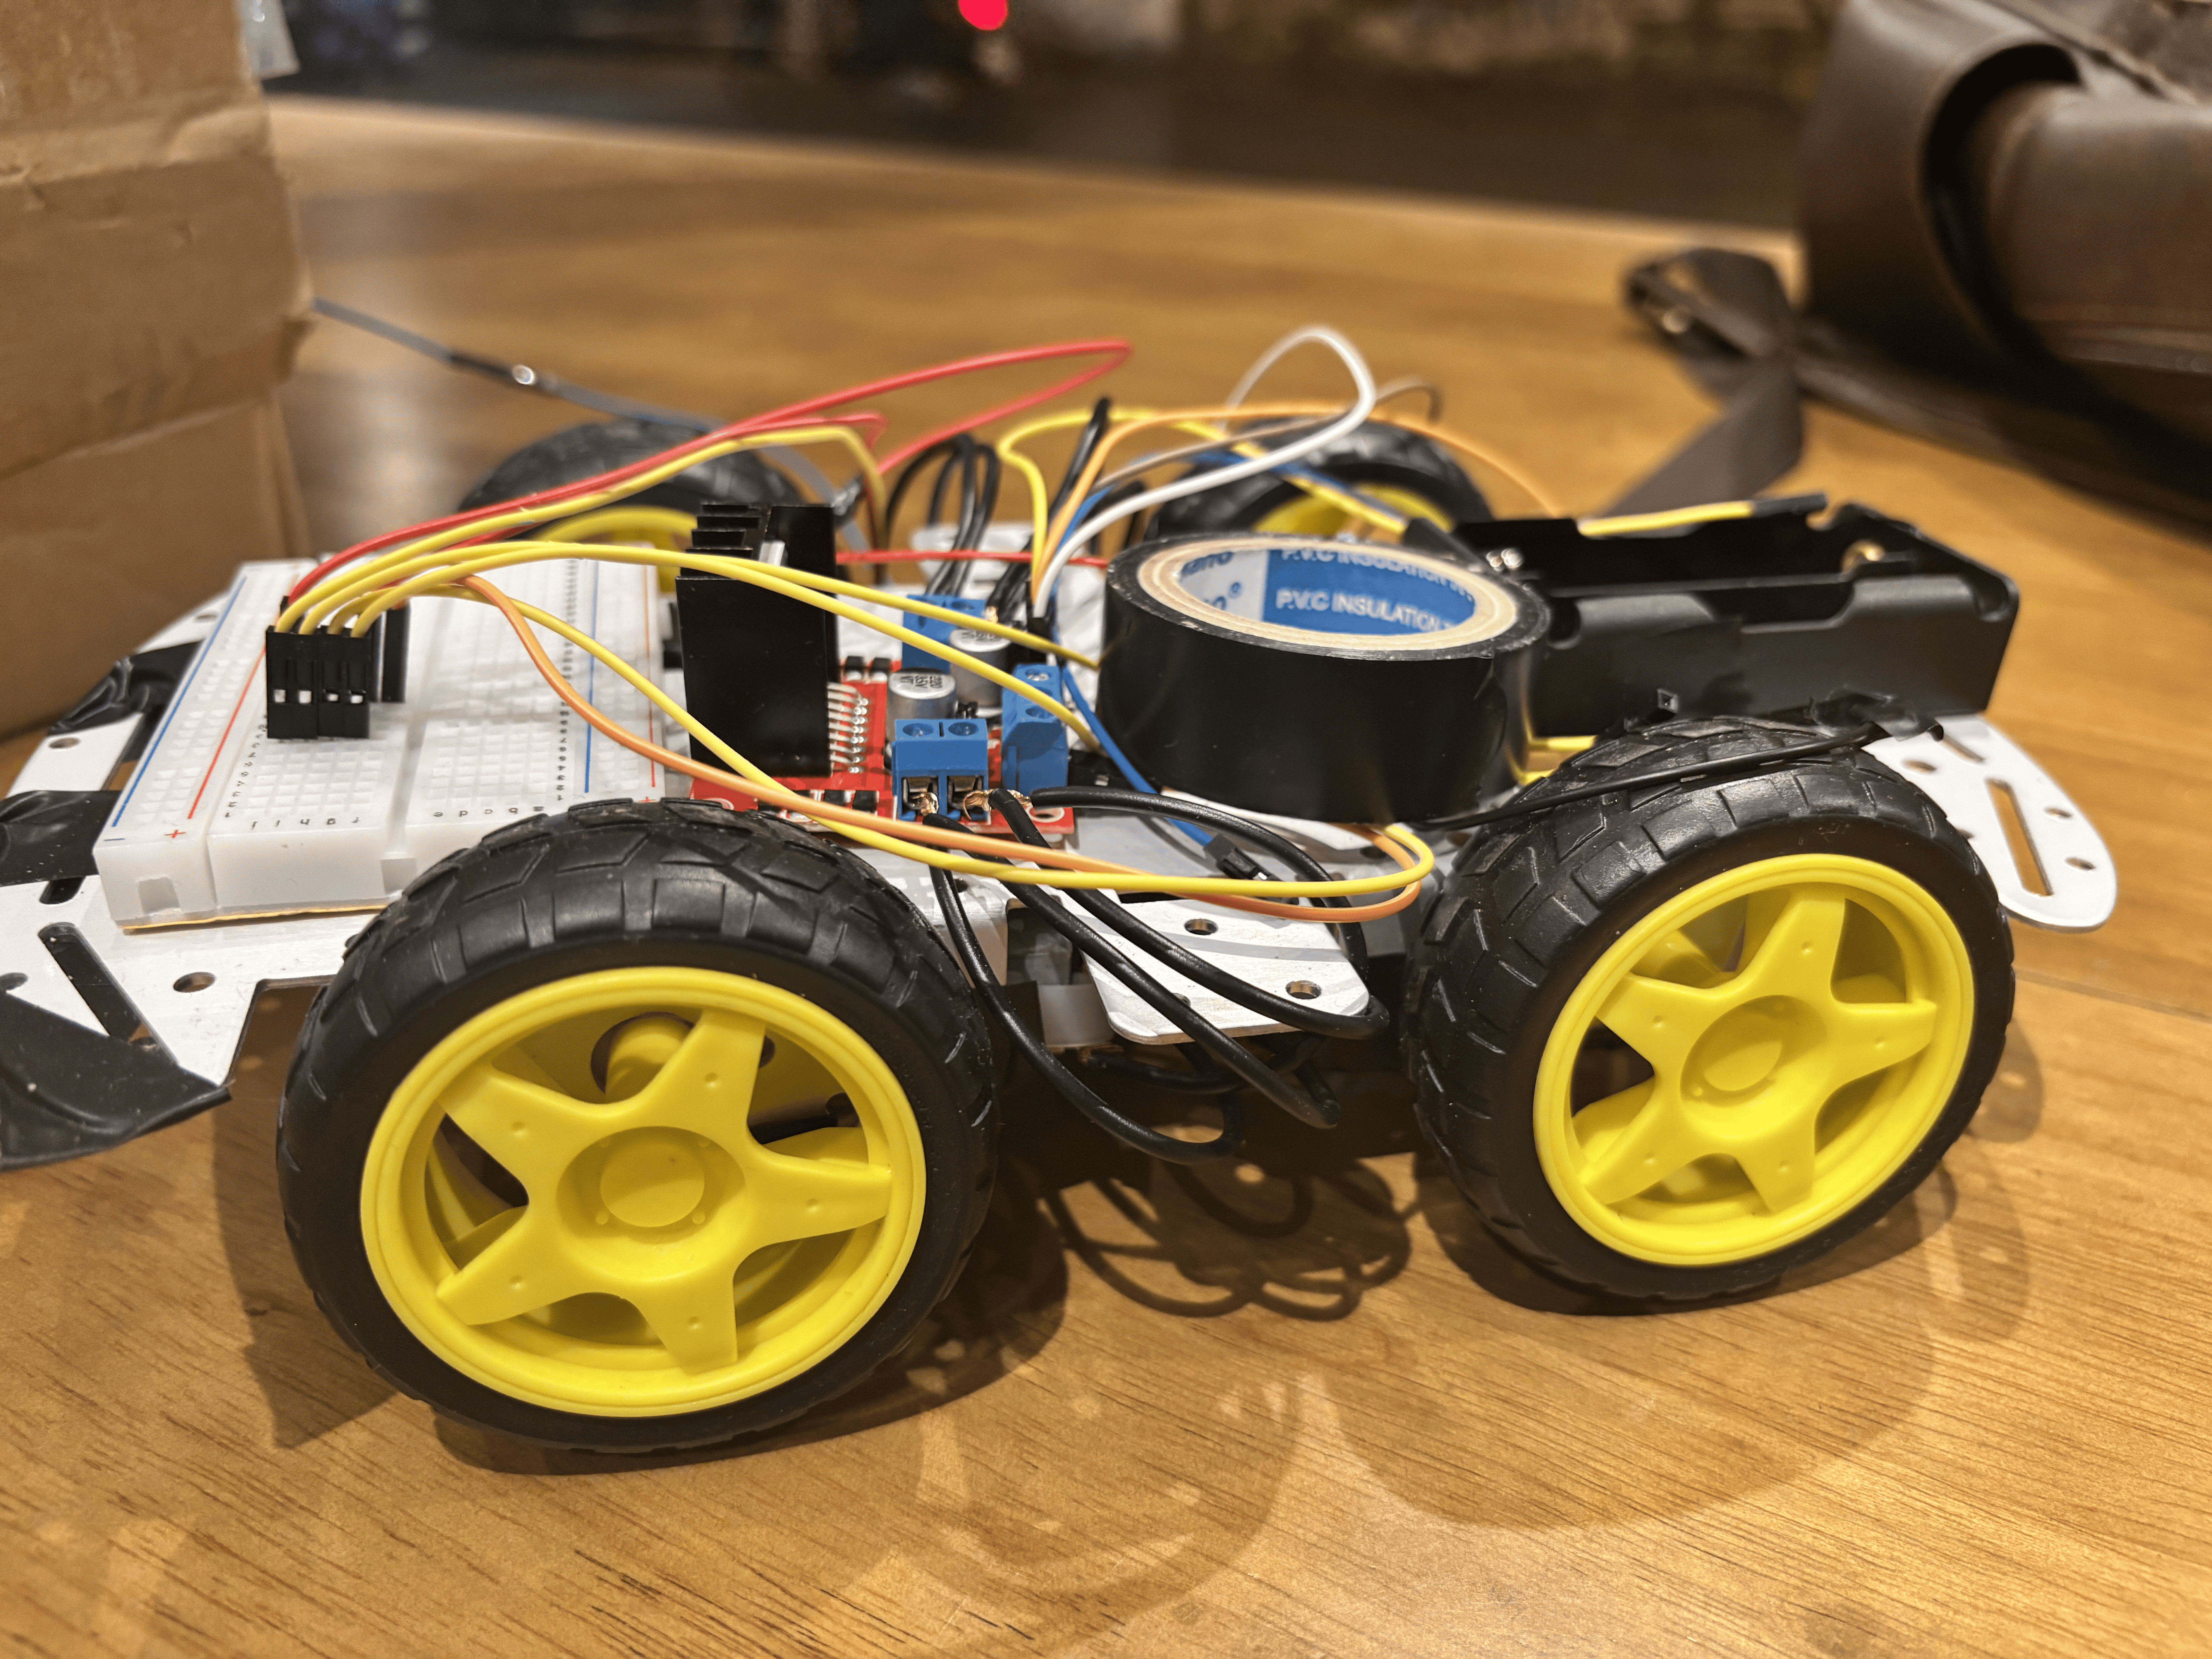
\includegraphics[width=\textwidth]{figures/hardware/rover_complete_photo.jpg}
    \fbox{\parbox{\textwidth}{\centering\vspace{5cm}FIGURE: Complete Rover Photograph\\Top-down view showing all components mounted on chassis\vspace{5cm}}}
    \caption{Fully assembled Rescue Rover showing the ESP32-S3 camera module, motor driver, battery, and chassis.}
    \label{fig:rover-complete}
\end{figure}

% --------------------------------------------------------
\section{Chassis Design}
\label{sec:chassis-design}

The chassis provides the structural foundation for all electronic components. We selected a commercially available tracked chassis platform rather than designing a custom frame. This decision saved significant development time while providing a proven mechanical platform.

\subsection{Platform Selection}

The selected chassis is a two-tracked tank-style platform with aluminum frame and plastic track segments. The tracked design was chosen over wheeled alternatives because tracks provide better traction on debris and can navigate over small obstacles that would stop wheels.

\begin{table}[h!]
    \centering
    \caption{Chassis specifications}
    \label{tab:chassis-specs}
    \begin{tabular}{ll}
        \toprule
        \textbf{Parameter} & \textbf{Value} \\
        \midrule
        Dimensions (L x W x H) & 150mm x 120mm x 45mm \\
        Weight (chassis only)  & 280g \\
        Material               & Aluminum frame, ABS tracks \\
        Track width            & 25mm \\
        Ground clearance       & 15mm \\
        Maximum load capacity  & 1.5 kg \\
        Motor mount            & Integrated DC motor brackets \\
        \bottomrule
    \end{tabular}
\end{table}

% FIGURE PLACEHOLDER
\begin{figure}[h!]
    \centering
    % \includegraphics[width=0.8\textwidth]{figures/hardware/chassis_dimensions.png}
    \fbox{\parbox{0.8\textwidth}{\centering\vspace{3.5cm}FIGURE: Chassis Dimensions Drawing\\Technical drawing with all measurements labeled\vspace{3.5cm}}}
    \caption{Chassis dimensional drawing showing mounting hole positions and overall dimensions.}
    \label{fig:chassis-dimensions}
\end{figure}

\subsection{Track Configuration}

The tracks use a timing belt design with tensioning idlers at each end. Tension is adjustable through slotted mounting holes. Proper tension is critical for reliable operation. Too loose and the track slips under load. Too tight and motor current increases significantly.

% FIGURE PLACEHOLDER
\begin{figure}[h!]
    \centering
    % \includegraphics[width=0.7\textwidth]{figures/hardware/track_detail.jpg}
    \fbox{\parbox{0.7\textwidth}{\centering\vspace{3cm}FIGURE: Track Detail Photograph\\Close-up showing track teeth, drive sprocket, and tensioner\vspace{3cm}}}
    \caption{Track assembly detail showing the drive sprocket, track segments, and tension adjustment mechanism.}
    \label{fig:track-detail}
\end{figure}

\subsection{Component Mounting}

Electronic components are mounted to the chassis using nylon standoffs and M3 screws. This approach allows easy removal for debugging and replacement. Components are arranged to balance weight distribution between the front and rear axles.

% FIGURE PLACEHOLDER
\begin{figure}[h!]
    \centering
    % \includegraphics[width=\textwidth]{figures/hardware/component_layout.png}
    \fbox{\parbox{\textwidth}{\centering\vspace{4cm}FIGURE: Component Layout Diagram\\Top-down view showing positions of ESP32-S3, L298N, battery, ultrasonic sensor\vspace{4cm}}}
    \caption{Component layout showing the physical arrangement of electronics on the chassis.}
    \label{fig:component-layout}
\end{figure}

% --------------------------------------------------------
\section{Main Controller: ESP32-S3}
\label{sec:esp32-controller}

The ESP32-S3 serves as the central processing unit for the rover. This chip was selected for its combination of processing power, wireless capabilities, camera interface, and extensive Arduino ecosystem support.

\subsection{Chip Specifications}

The ESP32-S3 is Espressif's third generation WiFi/Bluetooth microcontroller. It features dual Xtensa LX7 cores running at up to 240 MHz, significantly more powerful than the original ESP32.

\begin{table}[h!]
    \centering
    \caption{ESP32-S3 technical specifications}
    \label{tab:esp32-specs}
    \begin{tabular}{ll}
        \toprule
        \textbf{Feature} & \textbf{Specification} \\
        \midrule
        CPU           & Dual Xtensa LX7, up to 240 MHz \\
        SRAM          & 512 KB internal \\
        PSRAM         & 8 MB external (OPI interface) \\
        Flash         & 16 MB (QSPI) \\
        WiFi          & 802.11 b/g/n, 2.4 GHz \\
        Bluetooth     & LE 5.0 with coded PHY \\
        GPIO          & 45 programmable pins \\
        Camera        & DVP interface, up to 2MP \\
        USB           & USB 2.0 OTG \\
        Operating voltage & 3.0-3.6V (LDO regulates from 5V)\\
        \bottomrule
    \end{tabular}
\end{table}

% FIGURE PLACEHOLDER
\begin{figure}[h!]
    \centering
    % \includegraphics[width=0.7\textwidth]{figures/hardware/esp32s3_module_photo.jpg}
    \fbox{\parbox{0.7\textwidth}{\centering\vspace{3cm}FIGURE: ESP32-S3 Module Photograph\\Shows the development board with camera connector and USB-C port\vspace{3cm}}}
    \caption{ESP32-S3 WROOM development board used in the Rescue Rover.}
    \label{fig:esp32-module}
\end{figure}

\subsection{Development Board Selection}

Several ESP32-S3 development boards were evaluated. The Freenove ESP32-S3 WROOM was selected for its integrated camera connector, adequate PSRAM, and reasonable price point. Other options considered included the official Espressif DevKitC and the AI-Thinker ESP32-S3 CAM.

\begin{table}[h!]
    \centering
    \caption{ESP32-S3 development board comparison}
    \label{tab:board-comparison}
    \begin{tabular}{lccc}
        \toprule
        \textbf{Feature} & \textbf{Freenove} & \textbf{ESP32-CAM} & \textbf{DevKitC} \\
        \midrule
        PSRAM             & 8 MB  & 4 MB  & 8 MB \\
        Camera connector  & Yes   & Yes   & No \\
        Available GPIO    & 35+   & 10    & 45 \\
        USB programming   & Built-in & External & Built-in \\
        Price             & \$12  & \$8   & \$15 \\
        Selected          & Yes   & No    & No \\
        \bottomrule
    \end{tabular}
\end{table}

The ESP32-CAM was rejected despite its lower cost because of severe GPIO limitations. Many pins are shared between the camera, SD card, and flash, leaving insufficient pins for motor control and sensors.

% FIGURE PLACEHOLDER
\begin{figure}[h!]
    \centering
    % \includegraphics[width=\textwidth]{figures/hardware/board_comparison.png}
    \fbox{\parbox{\textwidth}{\centering\vspace{3.5cm}FIGURE: Development Board Comparison\\Side-by-side photos of evaluated boards with GPIO counts labeled\vspace{3.5cm}}}
    \caption{Comparison of evaluated development boards showing physical differences and GPIO availability.}
    \label{fig:board-comparison}
\end{figure}

\subsection{PSRAM Importance}

External PSRAM is essential for camera operation. Each QVGA frame requires 153.6 KB of buffer space. Double buffering doubles this requirement. Without PSRAM, the internal 512 KB SRAM would be exhausted by camera buffers alone, leaving no memory for the application.

The PSRAM connects via OPI (Octal Peripheral Interface) rather than QPI (Quad). OPI provides higher bandwidth, supporting faster frame transfers from the camera peripheral to the CPU.

% --------------------------------------------------------
\section{Camera System}
\label{sec:camera-hardware}

The camera provides the rover's primary sensing capability. Visual data is used for remote operation, obstacle detection, and AI scene analysis.

\subsection{OV2640 Sensor}

The OV2640 is a 2-megapixel CMOS image sensor commonly used in embedded vision applications. It connects to the ESP32-S3 through the DVP (Digital Video Port) parallel interface.

\begin{table}[h!]
    \centering
    \caption{OV2640 camera sensor specifications}
    \label{tab:ov2640-specs}
    \begin{tabular}{ll}
        \toprule
        \textbf{Parameter} & \textbf{Value} \\
        \midrule
        Resolution (max)   & 1600 x 1200 (2 MP) \\
        Output formats     & JPEG, YUV422, RGB565 \\
        Frame rate (SVGA)  & 30 FPS \\
        Frame rate (UXGA)  & 15 FPS \\
        Interface          & DVP (8-bit parallel) \\
        Control bus        & I2C (SCCB compatible) \\
        Operating voltage  & 2.5V core, 2.8V I/O \\
        Active pixels      & 1632 x 1232 \\
        Pixel size         & 2.2 x 2.2 $\mu$m \\
        \bottomrule
    \end{tabular}
\end{table}

% FIGURE PLACEHOLDER
\begin{figure}[h!]
    \centering
    % \includegraphics[width=0.5\textwidth]{figures/hardware/ov2640_module.jpg}
    \fbox{\parbox{0.5\textwidth}{\centering\vspace{2.5cm}FIGURE: OV2640 Camera Module\\Shows the module with lens and ribbon cable\vspace{2.5cm}}}
    \caption{OV2640 camera module showing the lens assembly and 24-pin FPC connector.}
    \label{fig:ov2640-module}
\end{figure}

\subsection{Resolution Selection}

The firmware configures the camera for QVGA (320 x 240) resolution rather than higher settings. This choice balances image quality against bandwidth and processing requirements. Higher resolutions would exceed UDP packet size limits and require frame fragmentation.

\begin{table}[h!]
    \centering
    \caption{Resolution trade-offs}
    \label{tab:resolution-tradeoffs}
    \begin{tabular}{lcccc}
        \toprule
        \textbf{Resolution} & \textbf{Pixels} & \textbf{JPEG Size} & \textbf{UDP OK} & \textbf{Selected} \\
        \midrule
        QQVGA (160x120) & 19,200    & 2-5 KB   & Yes & No (too small) \\
        QVGA (320x240)  & 76,800    & 5-15 KB  & Yes & Yes \\
        VGA (640x480)   & 307,200   & 20-50 KB & No  & No \\
        SVGA (800x600)  & 480,000   & 40-80 KB & No  & No \\
        \bottomrule
    \end{tabular}
\end{table}

% FIGURE PLACEHOLDER
\begin{figure}[h!]
    \centering
    % \includegraphics[width=\textwidth]{figures/hardware/resolution_comparison.png}
    \fbox{\parbox{\textwidth}{\centering\vspace{3.5cm}FIGURE: Resolution Comparison\\Sample frames at each resolution showing detail levels\vspace{3.5cm}}}
    \caption{Visual comparison of different camera resolutions showing the quality versus size trade-off.}
    \label{fig:resolution-comparison}
\end{figure}

\subsection{Lens and Field of View}

The camera module uses a wide-angle lens with approximately 120 degree horizontal field of view. Wide angle coverage is important for obstacle detection at close range. A narrow lens would create blind spots immediately in front of the rover.

% FIGURE PLACEHOLDER
\begin{figure}[h!]
    \centering
    % \includegraphics[width=0.7\textwidth]{figures/hardware/camera_fov.png}
    \fbox{\parbox{0.7\textwidth}{\centering\vspace{3cm}FIGURE: Camera Field of View Diagram\\Top-down view showing FOV cone relative to rover body\vspace{3cm}}}
    \caption{Camera field of view coverage showing the visibility area in front of the rover.}
    \label{fig:camera-fov}
\end{figure}

\subsection{Camera Mounting}

The camera is mounted at the front of the chassis, tilted downward by approximately 15 degrees. This angle provides visibility of both the immediate ground surface and obstacles at medium distance. The mount uses a 3D printed bracket that allows angle adjustment.

% FIGURE PLACEHOLDER
\begin{figure}[h!]
    \centering
    % \includegraphics[width=0.6\textwidth]{figures/hardware/camera_mount.jpg}
    \fbox{\parbox{0.6\textwidth}{\centering\vspace{3cm}FIGURE: Camera Mount Detail\\Shows 3D printed bracket and tilt angle\vspace{3cm}}}
    \caption{Camera mounting bracket showing the tilt angle and attachment method.}
    \label{fig:camera-mount}
\end{figure}

% --------------------------------------------------------
\section{Motor Control System}
\label{sec:motor-system}

The motor system provides locomotive power through two DC gear motors, one for each track. The L298N dual H-bridge driver controls motor direction and speed based on commands from the ESP32-S3.

\subsection{DC Gear Motors}

The motors are brushed DC type with integrated planetary gearboxes. The gearbox reduces output speed while increasing torque, essential for moving the chassis against friction and over obstacles.

\begin{table}[h!]
    \centering
    \caption{Motor specifications}
    \label{tab:motor-specs}
    \begin{tabular}{ll}
        \toprule
        \textbf{Parameter} & \textbf{Value} \\
        \midrule
        Nominal voltage    & 6-12V DC \\
        No-load speed      & 150 RPM at 12V \\
        Stall torque       & 3 kg-cm \\
        Stall current      & 1.5 A \\
        Operating current  & 200-500 mA \\
        Gear ratio         & 1:48 \\
        Shaft diameter     & 6 mm (D-cut) \\
        \bottomrule
    \end{tabular}
\end{table}

% FIGURE PLACEHOLDER
\begin{figure}[h!]
    \centering
    % \includegraphics[width=0.5\textwidth]{figures/hardware/dc_motor_gearbox.jpg}
    \fbox{\parbox{0.5\textwidth}{\centering\vspace{2.5cm}FIGURE: DC Gear Motor Photo\\Shows motor body, gearbox, and output shaft\vspace{2.5cm}}}
    \caption{DC gear motor showing the motor body, planetary gearbox, and output shaft.}
    \label{fig:motor-photo}
\end{figure}

\subsection{L298N Motor Driver}

The L298N is a dual full-bridge driver IC. Each bridge can deliver up to 2A continuous current, sufficient for our motors which draw 500mA under load. The module includes an onboard 5V regulator that powers the ESP32-S3.

\begin{table}[h!]
    \centering
    \caption{L298N specifications}
    \label{tab:l298n-specs}
    \begin{tabular}{ll}
        \toprule
        \textbf{Parameter} & \textbf{Value} \\
        \midrule
        Motor supply voltage & 5-35V \\
        Logic supply         & 5V (from onboard regulator or external) \\
        Per channel current  & 2A continuous, 3A peak \\
        Total power          & 25W max \\
        Control inputs       & 4 (IN1-IN4) \\
        Enable inputs        & 2 (ENA, ENB) \\
        Voltage drop         & 1.8V typical (at rated current) \\
        \bottomrule
    \end{tabular}
\end{table}

% FIGURE PLACEHOLDER
\begin{figure}[h!]
    \centering
    % \includegraphics[width=0.6\textwidth]{figures/hardware/l298n_module.jpg}
    \fbox{\parbox{0.6\textwidth}{\centering\vspace{3cm}FIGURE: L298N Motor Driver Board\\Shows input terminals, motor outputs, and heatsink\vspace{3cm}}}
    \caption{L298N motor driver module with the characteristic large heatsink and terminal blocks.}
    \label{fig:l298n-module}
\end{figure}

\subsection{L298N vs TB6612FNG}

During component selection, we compared the L298N against the more modern TB6612FNG. The TB6612 offers higher efficiency (90\% vs 70\%) due to MOSFET switching rather than bipolar transistors. However, the L298N was selected because of its higher current capacity and integrated voltage regulator.

\begin{table}[h!]
    \centering
    \caption{Motor driver comparison}
    \label{tab:driver-comparison}
    \begin{tabular}{lcc}
        \toprule
        \textbf{Feature} & \textbf{L298N} & \textbf{TB6612FNG} \\
        \midrule
        Max current     & 2A    & 1.2A \\
        Efficiency      & 70\%  & 90\% \\
        Voltage drop    & 1.8V  & 0.3V \\
        Heat generation & High  & Low \\
        5V regulator    & Built-in & None \\
        Cost            & \$3   & \$5 \\
        Selected        & Yes   & No \\
        \bottomrule
    \end{tabular}
\end{table}

The lower efficiency of the L298N means more power is dissipated as heat. For extended operation, the heatsink temperature can exceed 60 degrees Celsius. Future revisions may switch to the TB6612 if thermal throttling becomes problematic.

% FIGURE PLACEHOLDER
\begin{figure}[h!]
    \centering
    % 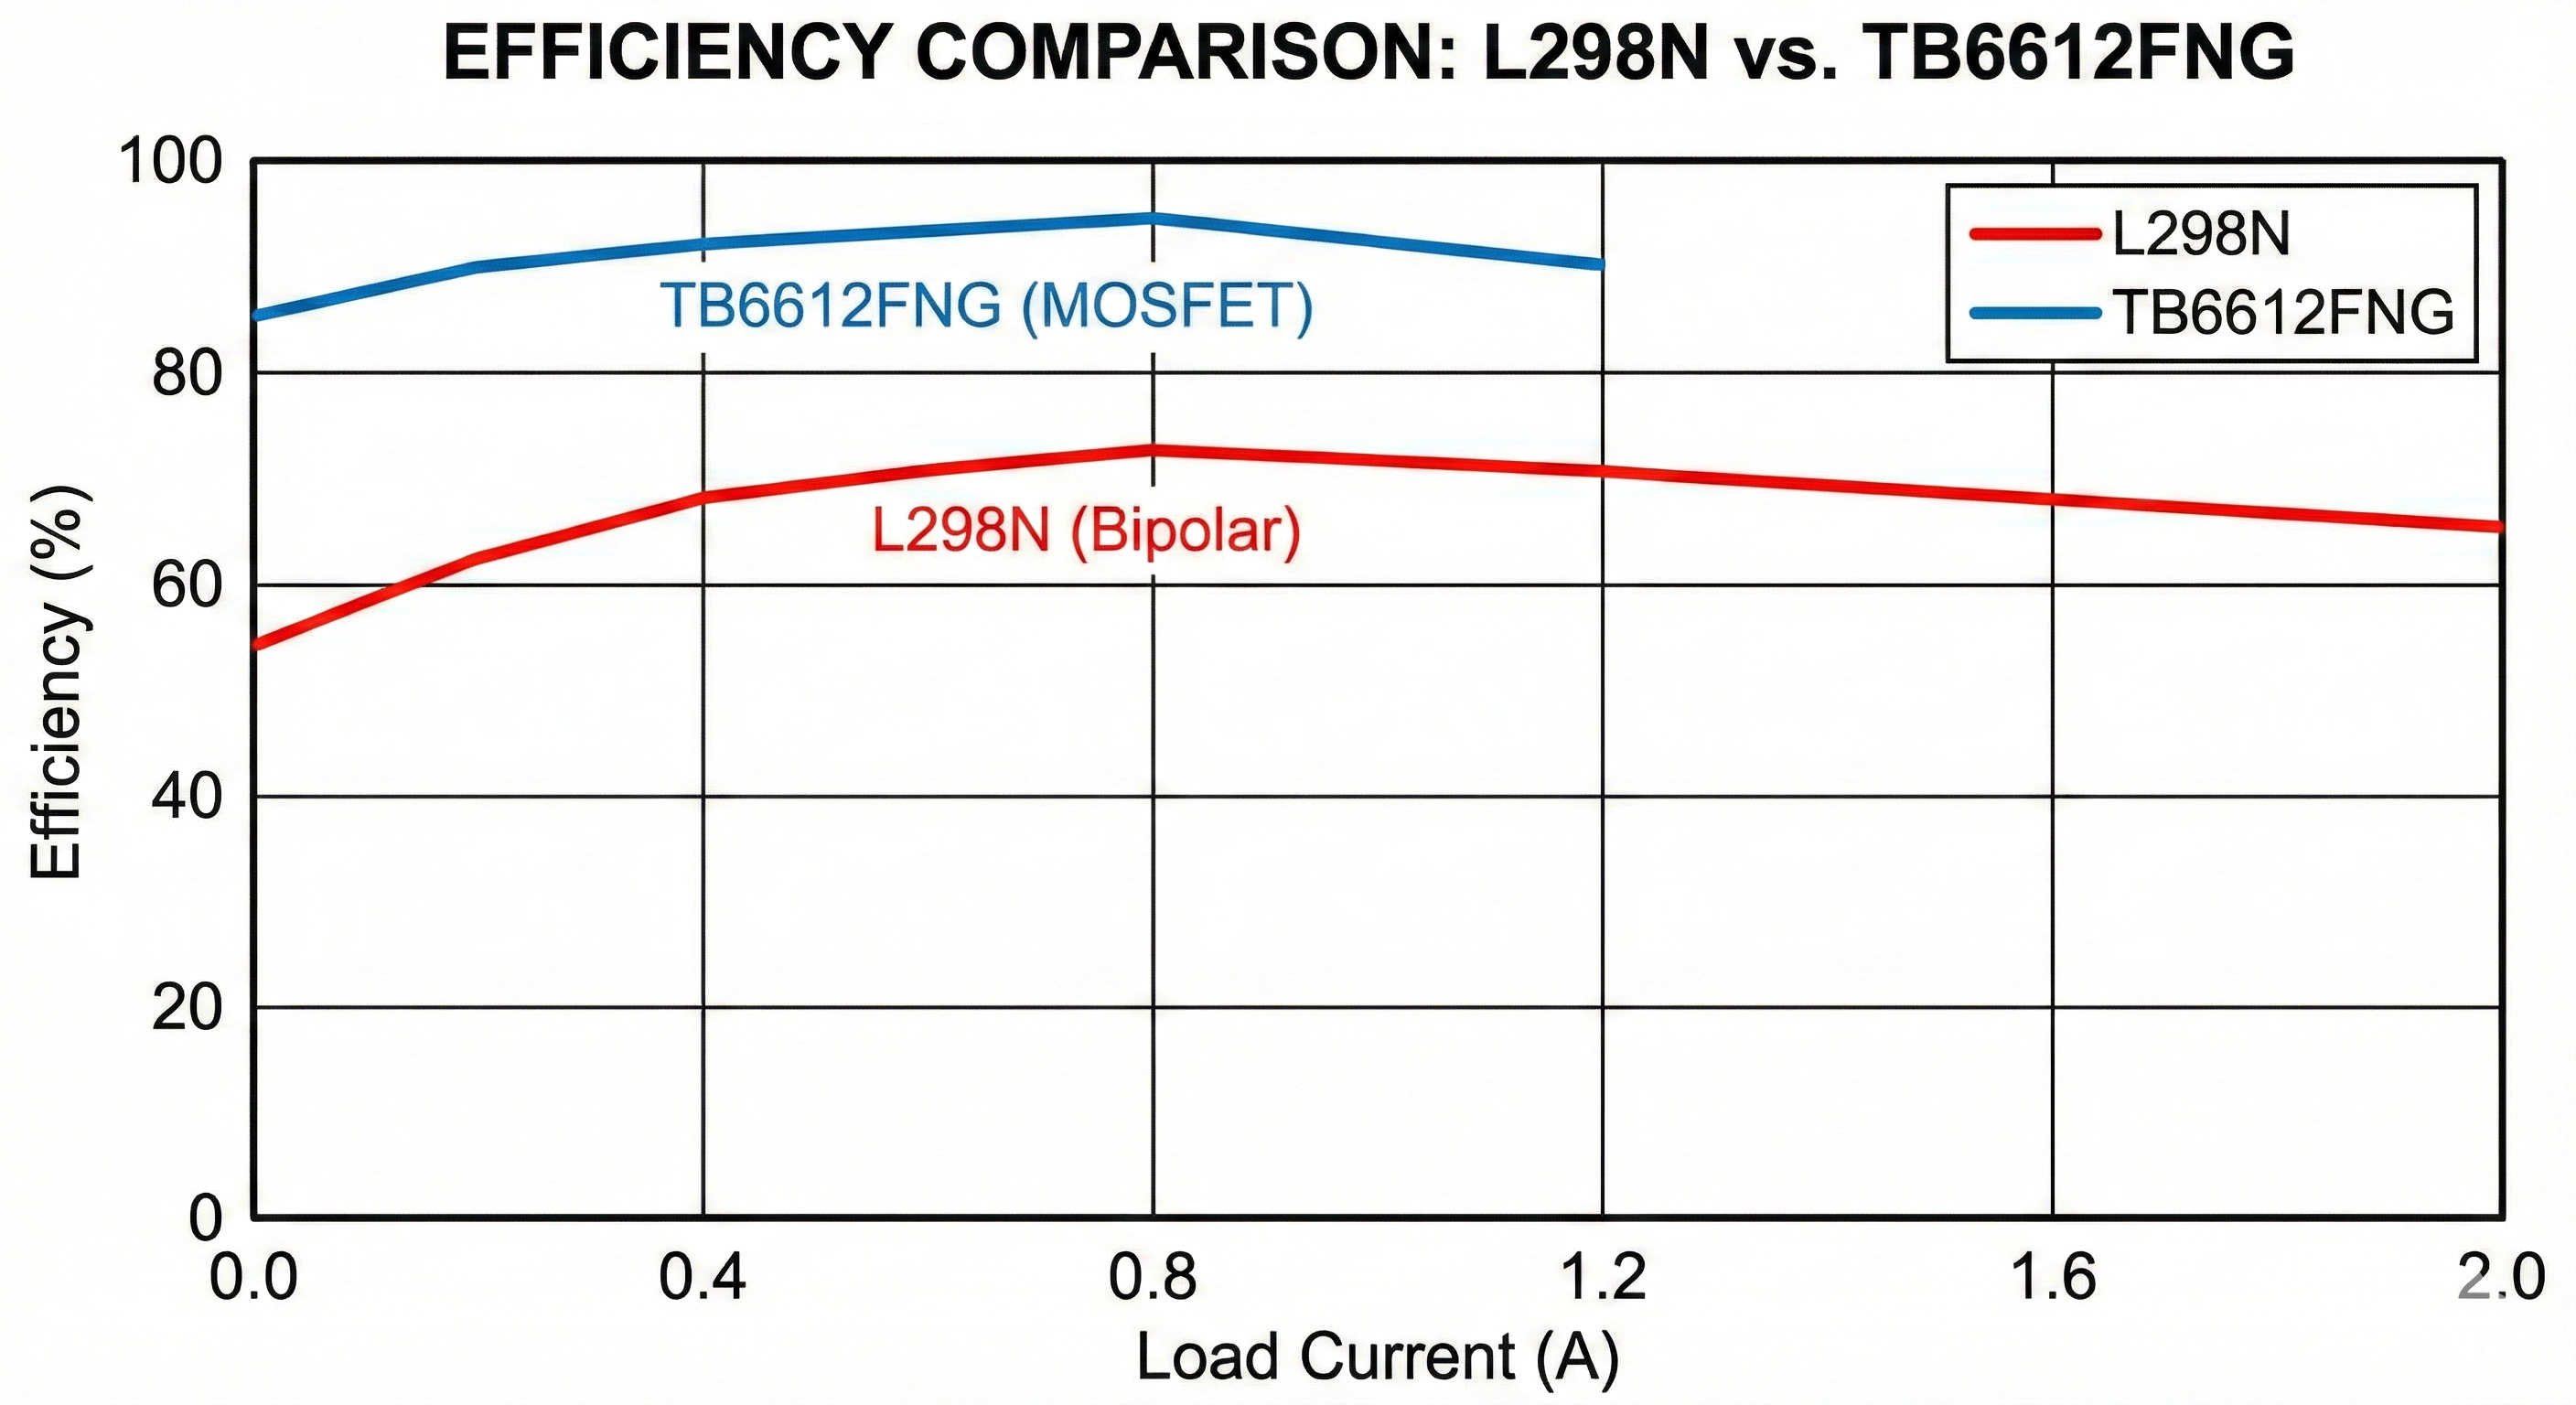
\includegraphics[width=0.8\textwidth]{figures/charts/driver_efficiency.png}
    \fbox{\parbox{0.8\textwidth}{\centering\vspace{3cm}FIGURE: Driver Efficiency Graph\\Current vs efficiency curves for both drivers\vspace{3cm}}}
    \caption{Efficiency comparison between L298N and TB6612FNG at various load currents.}
    \label{fig:efficiency-graph}
\end{figure}

% --------------------------------------------------------
\section{Power Distribution}
\label{sec:power-distribution}

The power system delivers appropriate voltages to all components from a single lithium polymer battery. Power management includes voltage regulation, protection circuits, and monitoring.

\subsection{Battery Selection}

A 3-cell (3S) lithium polymer battery provides the primary power. The 11.1V nominal voltage is compatible with both the motors (rated for 6-12V) and the L298N 5V regulator input range.

\begin{table}[h!]
    \centering
    \caption{Battery specifications}
    \label{tab:battery-specs}
    \begin{tabular}{ll}
        \toprule
        \textbf{Parameter} & \textbf{Value} \\
        \midrule
        Chemistry       & Lithium Polymer (LiPo) \\
        Configuration   & 3S (3 cells in series) \\
        Nominal voltage & 11.1V \\
        Fully charged   & 12.6V \\
        Low cutoff      & 9.9V (3.3V per cell) \\
        Capacity        & 2200 mAh \\
        Discharge rate  & 25C continuous \\
        Weight          & 180g \\
        \bottomrule
    \end{tabular}
\end{table}

% FIGURE PLACEHOLDER
\begin{figure}[h!]
    \centering
    % \includegraphics[width=0.5\textwidth]{figures/hardware/lipo_battery.jpg}
    \fbox{\parbox{0.5\textwidth}{\centering\vspace{2.5cm}FIGURE: LiPo Battery Photo\\Shows 3S pack with balance connector and XT60 plug\vspace{2.5cm}}}
    \caption{3S LiPo battery used to power the Rescue Rover.}
    \label{fig:battery-photo}
\end{figure}

\subsection{Power Budget}

The power budget analysis ensures the battery can supply all loads simultaneously. Total maximum draw is approximately 2.5A, well within the battery's 55A (25C x 2.2Ah) capability.

\begin{table}[h!]
    \centering
    \caption{System power budget}
    \label{tab:power-budget}
    \begin{tabular}{lccc}
        \toprule
        \textbf{Component} & \textbf{Voltage} & \textbf{Current (typ)} & \textbf{Current (max)} \\
        \midrule
        ESP32-S3 + Camera & 3.3V  & 300 mA  & 500 mA \\
        L298N quiescent   & 5V    & 36 mA   & 50 mA \\
        Left motor        & 12V   & 250 mA  & 1.5 A \\
        Right motor       & 12V   & 250 mA  & 1.5 A \\
        Ultrasonic sensor & 5V    & 15 mA   & 20 mA \\
        \midrule
        \textbf{Total}    & --    & 851 mA  & 3.57 A \\
        \bottomrule
    \end{tabular}
\end{table}

At typical consumption of 851 mA, the 2200 mAh battery provides approximately 2.5 hours of operation. Under maximum load (both motors stalled), runtime drops to approximately 40 minutes. Actual runtime during normal operation falls between these extremes.

% FIGURE PLACEHOLDER
\begin{figure}[h!]
    \centering
    % \includegraphics[width=\textwidth]{figures/hardware/power_distribution_diagram.png}
    \fbox{\parbox{\textwidth}{\centering\vspace{4cm}FIGURE: Power Distribution Schematic\\Shows battery, regulator, and all loads with current paths\vspace{4cm}}}
    \caption{Power distribution schematic showing voltage rails and current flow to all components.}
    \label{fig:power-schematic}
\end{figure}

\subsection{Voltage Regulation}

The L298N module includes a 78M05 linear regulator that provides 5V output from the 12V motor supply. This 5V rail powers the ESP32-S3 and ultrasonic sensor. The ESP32's internal LDO then produces 3.3V for the microcontroller core and camera.

% FIGURE PLACEHOLDER
\begin{figure}[h!]
    \centering
    % \includegraphics[width=0.7\textwidth]{figures/hardware/voltage_rails.png}
    \fbox{\parbox{0.7\textwidth}{\centering\vspace{2.5cm}FIGURE: Voltage Rail Diagram\\Shows 12V, 5V, and 3.3V rails with regulator symbols\vspace{2.5cm}}}
    \caption{Voltage rail hierarchy showing the cascade of regulators from battery to components.}
    \label{fig:voltage-rails}
\end{figure}

% --------------------------------------------------------
\section{Ultrasonic Distance Sensor}
\label{sec:ultrasonic-sensor}

The ultrasonic sensor provides proximity detection for obstacle avoidance. It measures the time of flight for a sound pulse to reach an obstacle and return.

\subsection{HC-SR04 Specifications}

\begin{table}[h!]
    \centering
    \caption{Ultrasonic sensor specifications}
    \label{tab:hcsr04-specs}
    \begin{tabular}{ll}
        \toprule
        \textbf{Parameter} & \textbf{Value} \\
        \midrule
        Operating voltage  & 5V DC \\
        Operating current  & 15 mA \\
        Frequency          & 40 kHz \\
        Range              & 2 cm to 400 cm \\
        Resolution         & 0.3 cm \\
        Measuring angle    & 15 degrees cone \\
        Trigger pulse      & 10 $\mu$s minimum \\
        \bottomrule
    \end{tabular}
\end{table}

% FIGURE PLACEHOLDER
\begin{figure}[h!]
    \centering
    % \includegraphics[width=0.5\textwidth]{figures/hardware/hcsr04_photo.jpg}
    \fbox{\parbox{0.5\textwidth}{\centering\vspace{2.5cm}FIGURE: HC-SR04 Sensor Photo\\Shows the sensor with two transducer cylinders\vspace{2.5cm}}}
    \caption{HC-SR04 ultrasonic distance sensor showing the transmitter and receiver transducers.}
    \label{fig:hcsr04-photo}
\end{figure}

\subsection{Mounting Position}

The sensor is mounted at the front of the chassis, below the camera. This position provides distance measurements along the rover's direction of travel. The narrow 15-degree beam angle means only obstacles directly ahead are detected. Side obstacles require camera based detection.

% FIGURE PLACEHOLDER
\begin{figure}[h!]
    \centering
    % \includegraphics[width=0.7\textwidth]{figures/hardware/ultrasonic_beam.png}
    \fbox{\parbox{0.7\textwidth}{\centering\vspace{3cm}FIGURE: Ultrasonic Beam Pattern\\Top-down view showing 15 degree detection cone\vspace{3cm}}}
    \caption{Ultrasonic beam pattern showing the narrow detection cone.}
    \label{fig:ultrasonic-beam}
\end{figure}

\subsection{Level Shifting}

The HC-SR04 operates at 5V logic levels while the ESP32-S3 GPIO pins are 3.3V. The echo pin outputs 5V, which could damage the ESP32 input. A simple resistor voltage divider scales the echo signal down to 3.3V safe levels.

\begin{lstlisting}[caption={Voltage divider calculation}]
R1 = 1kOhm, R2 = 2kOhm
V_out = V_in * R2 / (R1 + R2)
V_out = 5V * 2k / 3k = 3.33V
\end{lstlisting}

% FIGURE PLACEHOLDER
\begin{figure}[h!]
    \centering
    % \includegraphics[width=0.6\textwidth]{figures/hardware/level_shifter_circuit.png}
    \fbox{\parbox{0.6\textwidth}{\centering\vspace{2.5cm}FIGURE: Level Shifter Circuit\\Resistor divider schematic for ECHO pin\vspace{2.5cm}}}
    \caption{Resistor voltage divider for level shifting the 5V echo signal to 3.3V.}
    \label{fig:level-shifter}
\end{figure}

% --------------------------------------------------------
\section{Wiring and Interconnections}
\label{sec:wiring}

This section documents all electrical connections between components. Dupont jumper wires are used throughout for easy modification during development.

\subsection{Complete Wiring Diagram}

% FIGURE PLACEHOLDER
\begin{figure}[h!]
    \centering
    % \includegraphics[width=\textwidth]{figures/hardware/complete_wiring_diagram.png}
    \fbox{\parbox{\textwidth}{\centering\vspace{6cm}FIGURE: Complete Wiring Diagram\\Fritzing-style diagram showing all connections between components\vspace{6cm}}}
    \caption{Complete wiring diagram showing all connections between the ESP32-S3, L298N, motors, sensors, and power supply.}
    \label{fig:complete-wiring}
\end{figure}

\subsection{Wire Color Convention}

\begin{table}[h!]
    \centering
    \caption{Wire color coding standard}
    \label{tab:wire-colors}
    \begin{tabular}{ll}
        \toprule
        \textbf{Color} & \textbf{Purpose} \\
        \midrule
        Red    & Positive power (12V, 5V, 3.3V) \\
        Black  & Ground \\
        Yellow & Signal (GPIO outputs) \\
        Orange & Signal (GPIO inputs) \\
        Green  & I2C SDA \\
        Blue   & I2C SCL \\
        \bottomrule
    \end{tabular}
\end{table}

% FIGURE PLACEHOLDER
\begin{figure}[h!]
    \centering
    % \includegraphics[width=0.8\textwidth]{figures/hardware/wiring_photo.jpg}
    \fbox{\parbox{0.8\textwidth}{\centering\vspace{3.5cm}FIGURE: Actual Wiring Photograph\\Photo of real rover showing wire routing and organization\vspace{3.5cm}}}
    \caption{Actual wiring on the prototype showing careful routing and color coding.}
    \label{fig:wiring-photo}
\end{figure}

% --------------------------------------------------------
\section{Assembly Process}
\label{sec:assembly}

The complete assembly follows a specific order to ensure proper fit and cable routing.

\subsection{Assembly Steps}

\begin{enumerate}
    \item Mount motors to chassis brackets using M3 screws
    \item Attach drive sprockets to motor shafts
    \item Install tracks with proper tension
    \item Mount battery holder to rear platform
    \item Attach L298N driver with standoffs
    \item Mount ESP32-S3 board adjacent to L298N
    \item Install ultrasonic sensor at front
    \item Mount camera module on adjustable bracket
    \item Complete all wiring connections
    \item Verify connections with multimeter before power on
\end{enumerate}

% FIGURE PLACEHOLDER
\begin{figure}[h!]
    \centering
    % 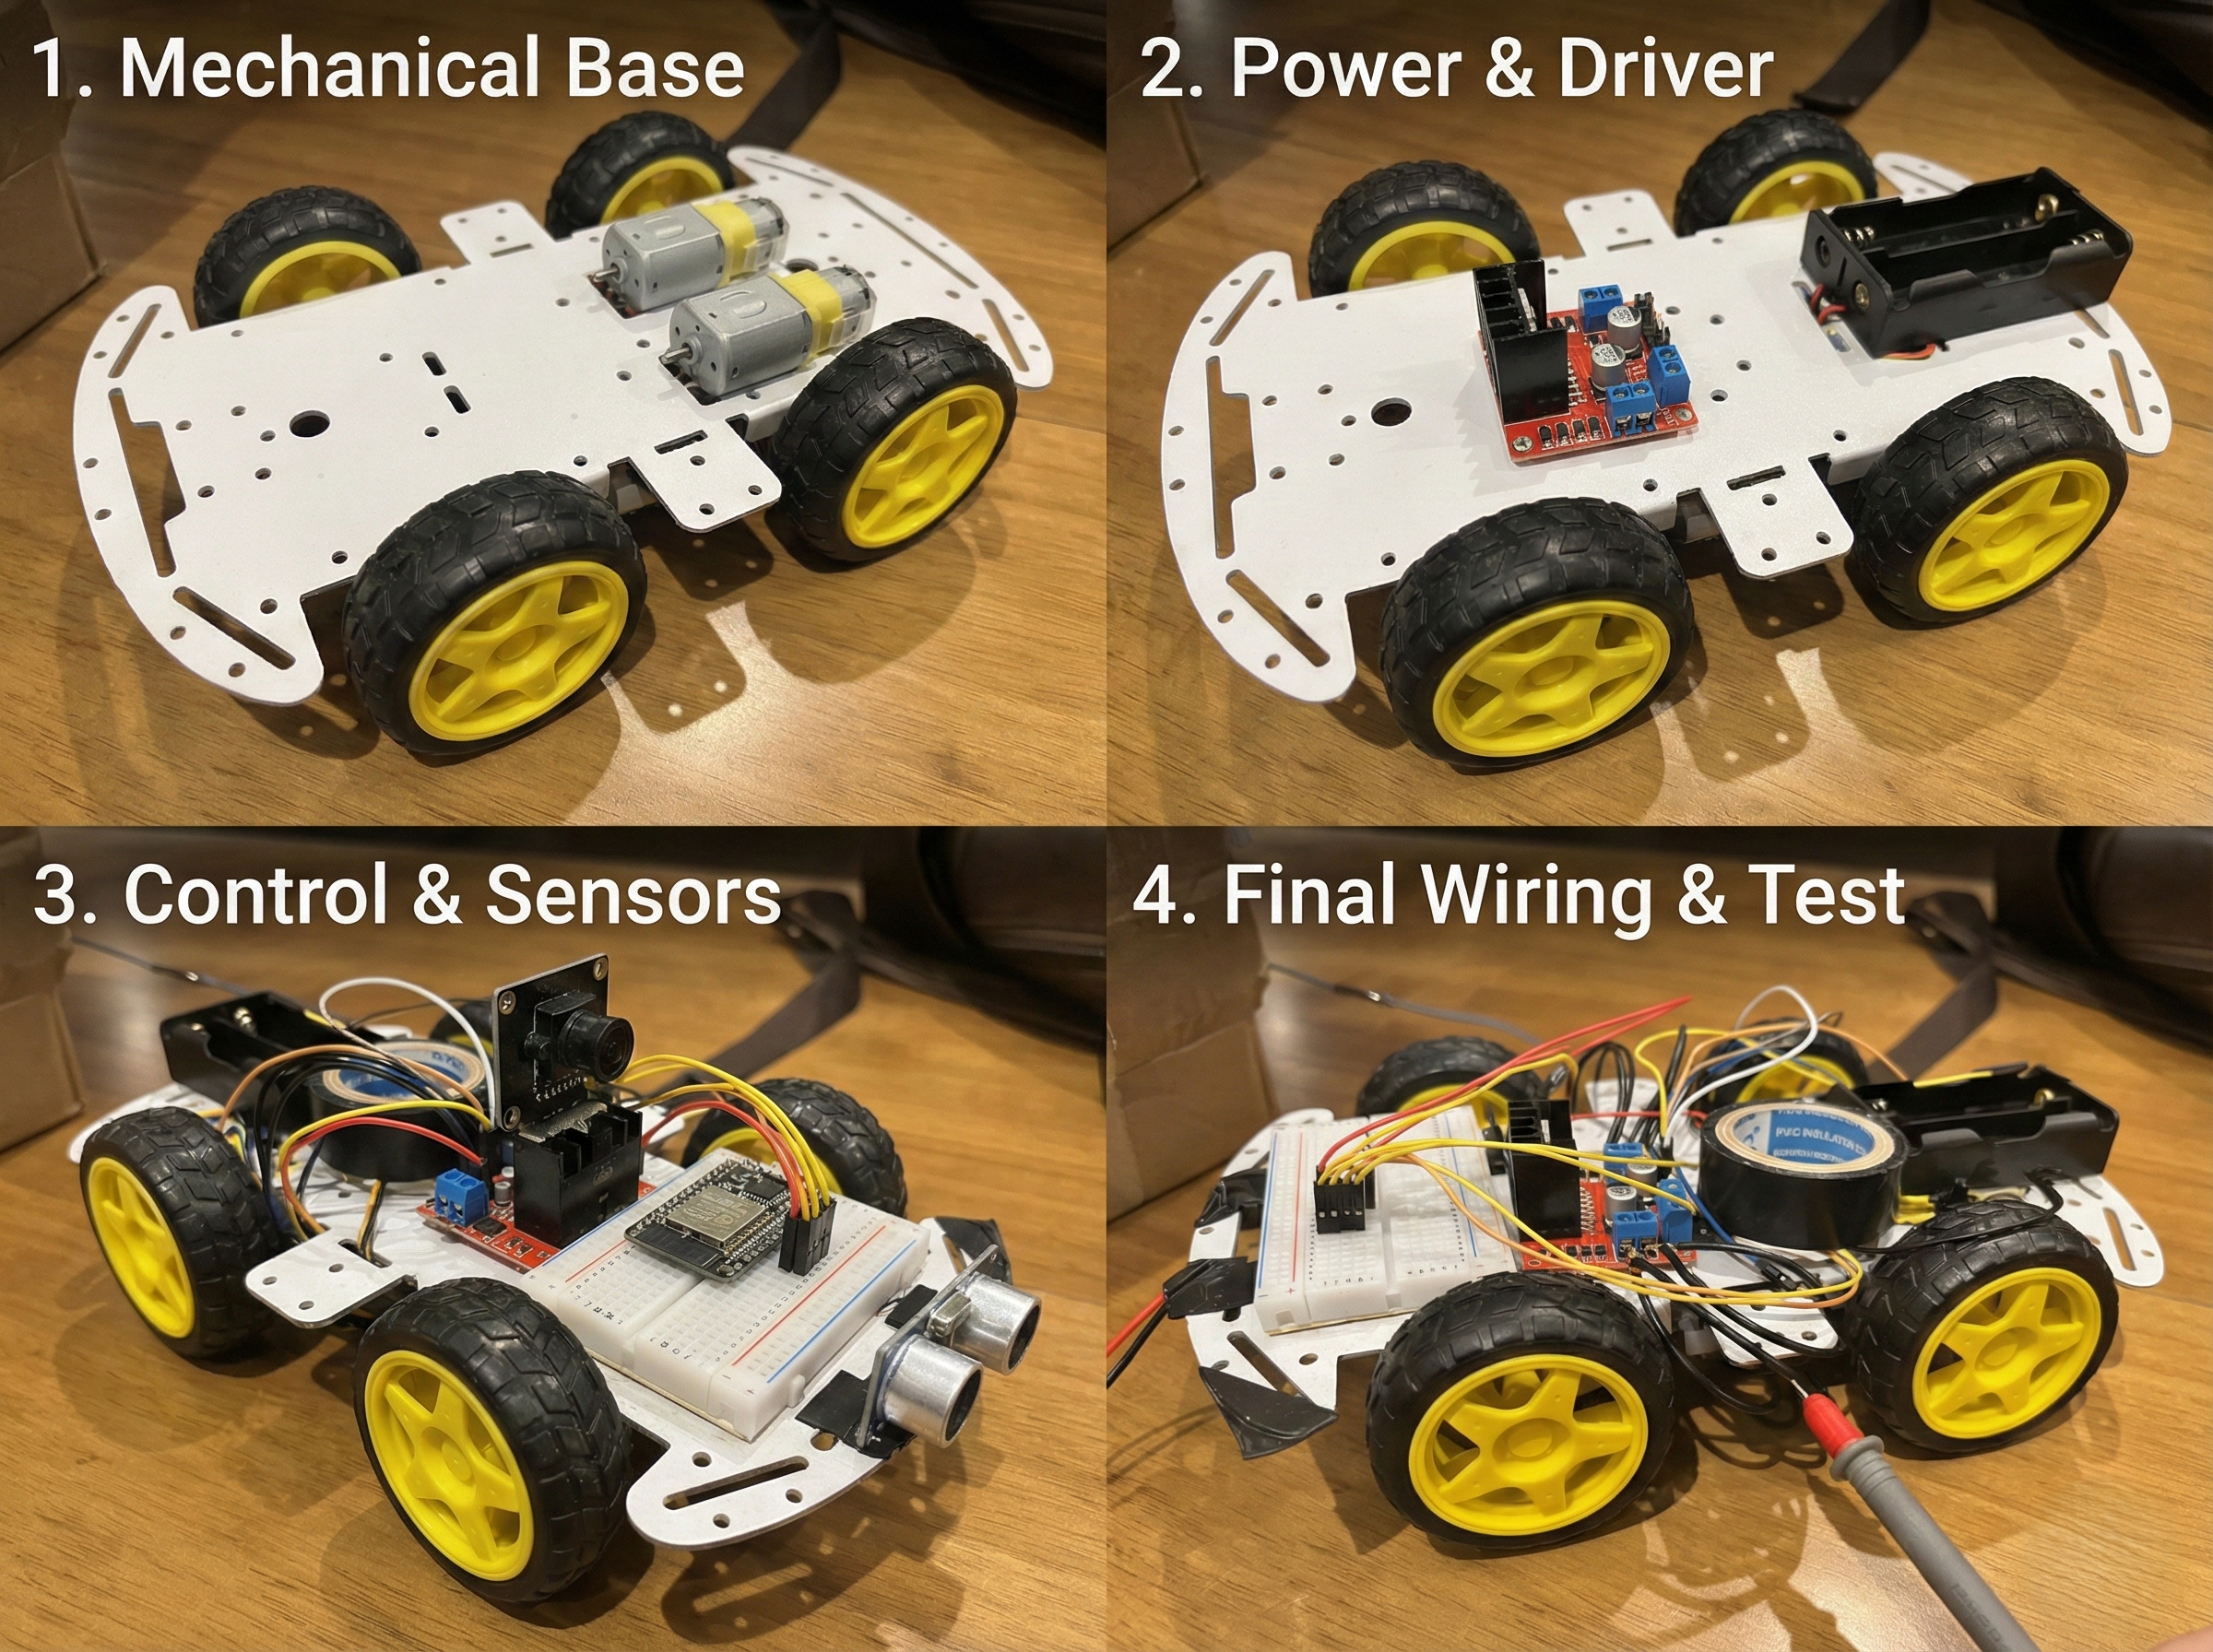
\includegraphics[width=\textwidth]{figures/hardware/assembly_sequence.png}
    \fbox{\parbox{\textwidth}{\centering\vspace{4cm}FIGURE: Assembly Sequence Photos\\Grid of 4-6 photos showing key assembly steps\vspace{4cm}}}
    \caption{Assembly sequence showing the progressive addition of components to the chassis.}
    \label{fig:assembly-sequence}
\end{figure}

\subsection{Testing Procedure}

After assembly, each subsystem is tested individually before full integration testing.

\begin{table}[h!]
    \centering
    \caption{Post-assembly test checklist}
    \label{tab:test-checklist}
    \begin{tabular}{lp{8cm}}
        \toprule
        \textbf{Subsystem} & \textbf{Test Procedure} \\
        \midrule
        Power     & Verify 5V and 3.3V rails with multimeter \\
        Motors    & Check rotation direction for each motor separately \\
        Camera    & Verify video feed appears in browser \\
        Ultrasonic & Move hand toward sensor, verify distance changes \\
        WiFi      & Confirm connection to access point \\
        ESP-NOW   & Verify command reception from gateway \\
        \bottomrule
    \end{tabular}
\end{table}

% FIGURE PLACEHOLDER
\begin{figure}[h!]
    \centering
    % 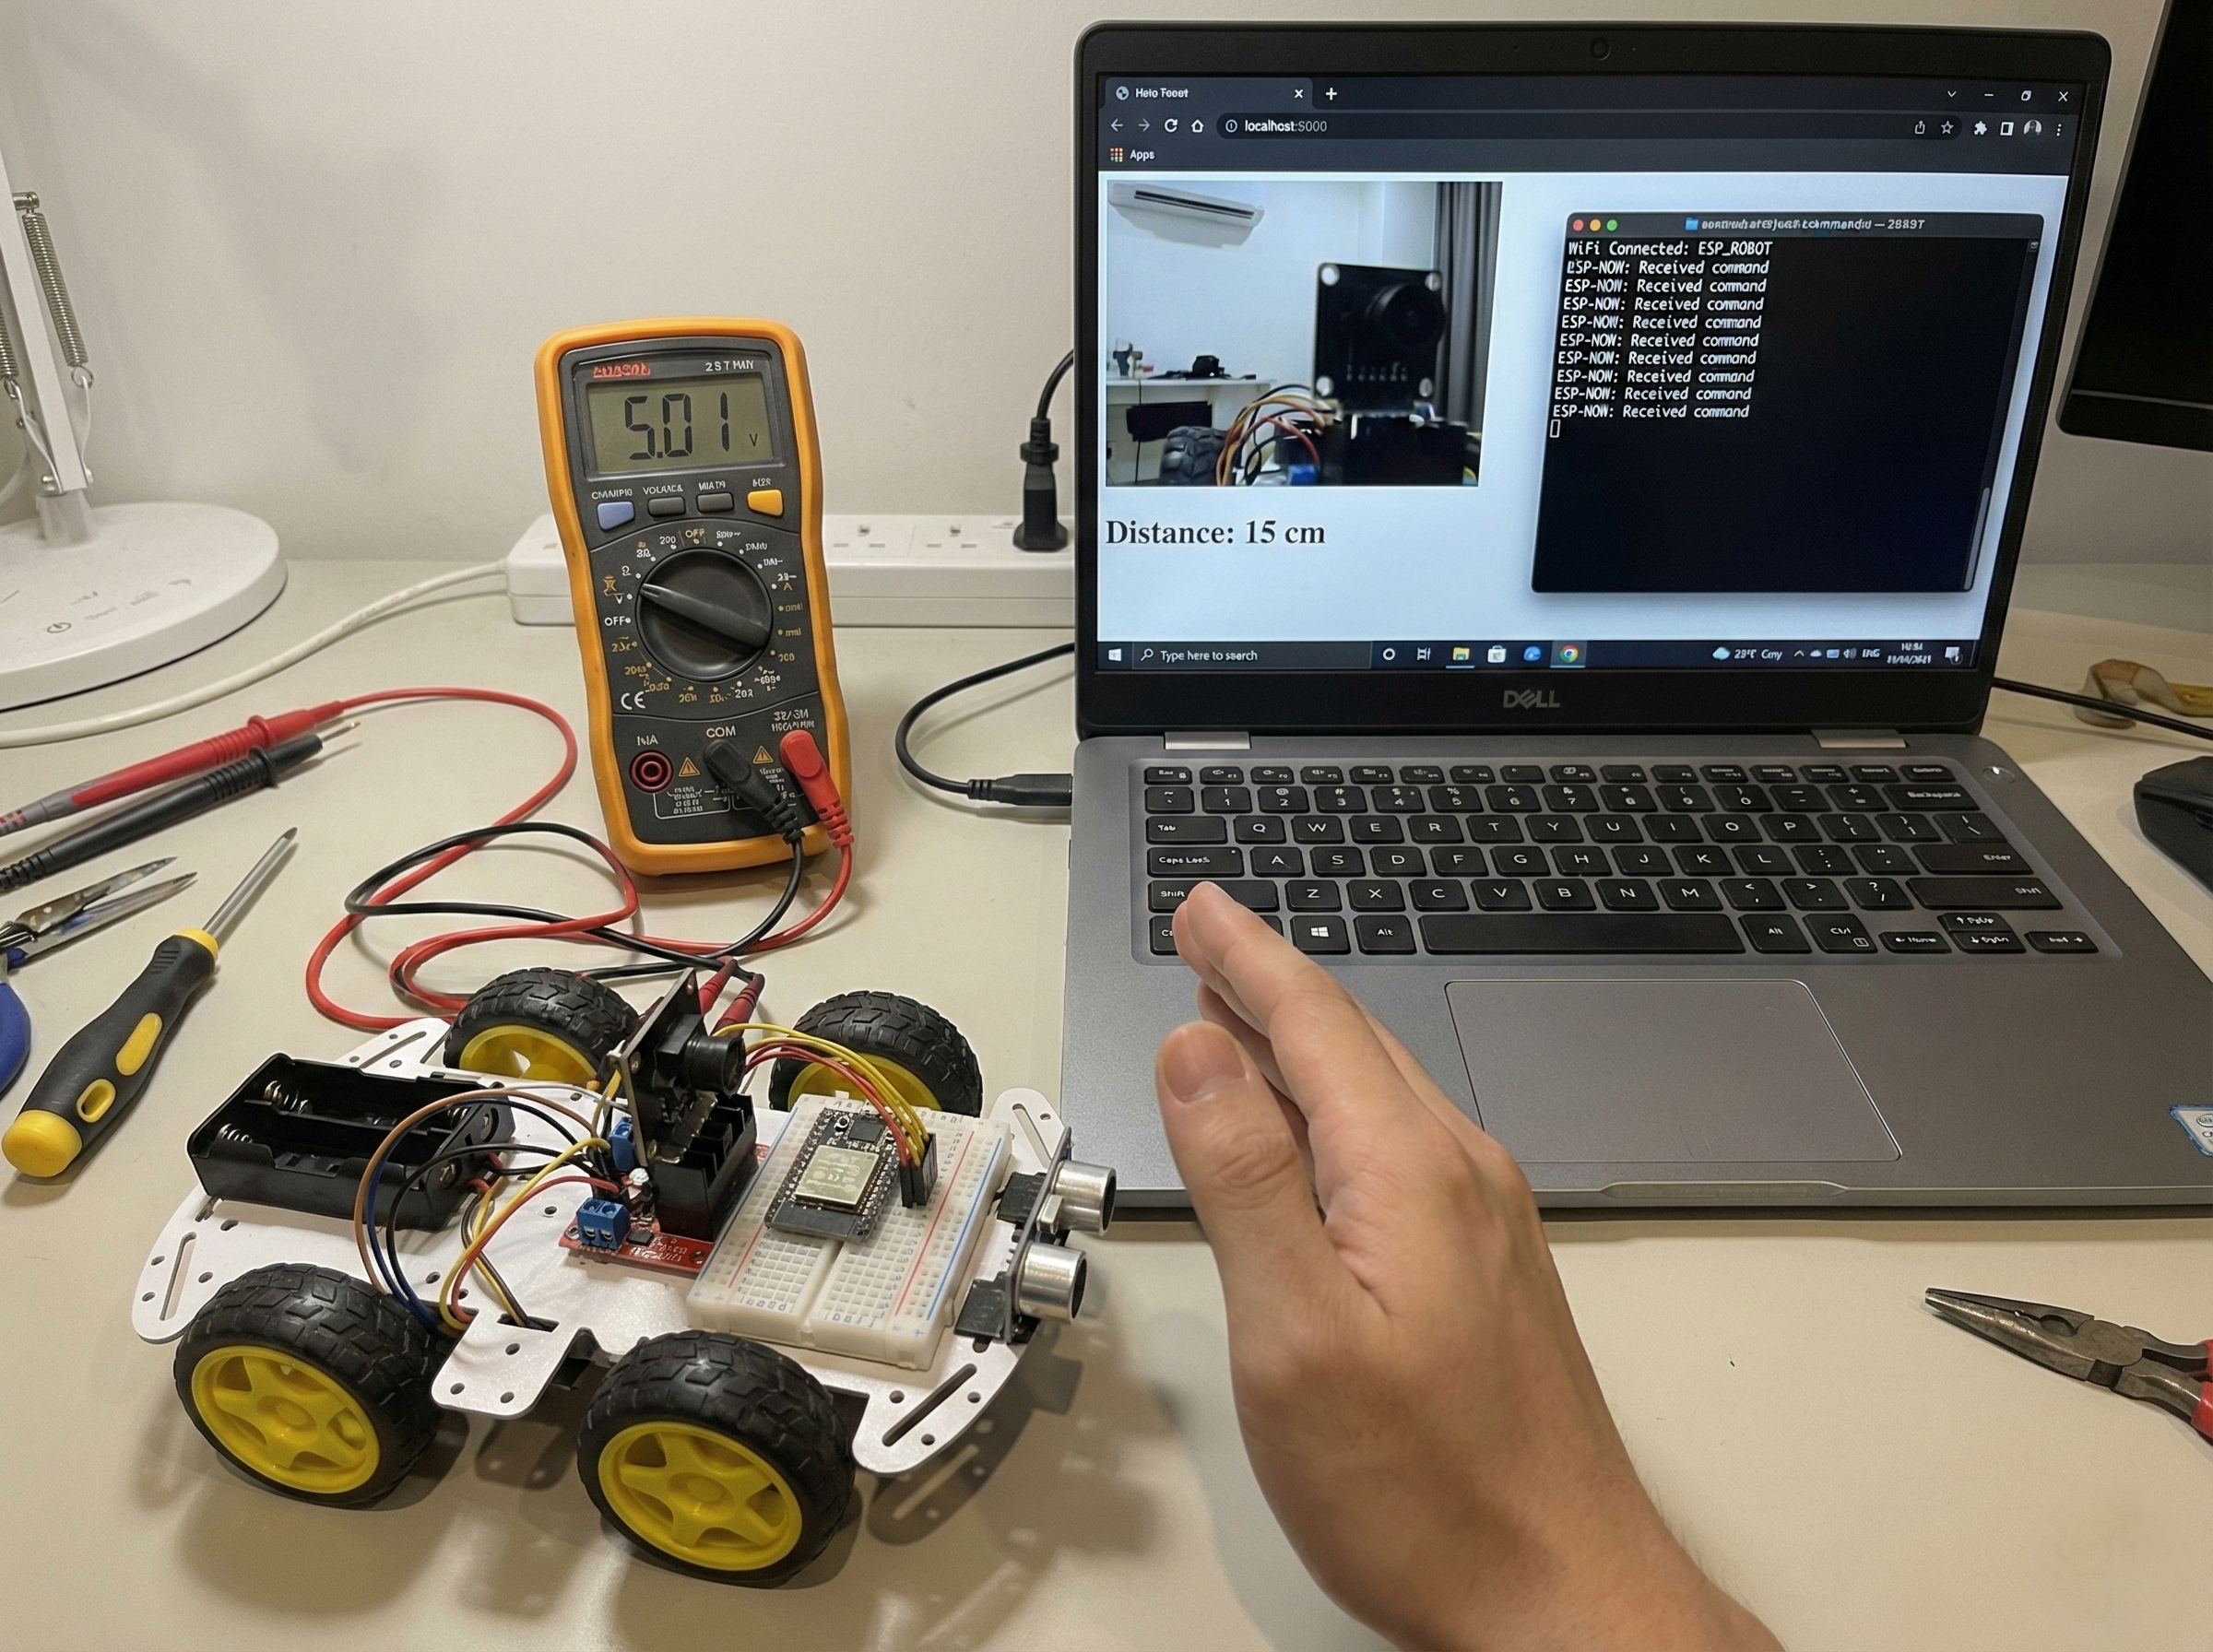
\includegraphics[width=0.7\textwidth]{figures/hardware/testing_setup.jpg}
    \fbox{\parbox{0.7\textwidth}{\centering\vspace{3cm}FIGURE: Testing Setup Photo\\Shows multimeter, test equipment, and rover on bench\vspace{3cm}}}
    \caption{Testing setup for post-assembly verification of subsystems.}
    \label{fig:testing-setup}
\end{figure}
